\documentclass[12pt,a4paper]{article}
\usepackage[utf8]{inputenc}
\usepackage[spanish]{babel}
\usepackage{amsmath,amssymb}
\usepackage{graphicx}
\usepackage{float}
\usepackage{hyperref}
\usepackage{geometry}
\usepackage{listings}
\usepackage{xcolor}

\geometry{margin=2.5cm}

\title{\textbf{Simulación de N Partículas en una Caja} \\ 
       \large Análisis de Dinámica Molecular y Teoría Cinética}
\author{[Tu Nombre] \\ [Nombre del Compañero] \\
        \small Física Computacional 2 \\
        \small Profesor: John Hernán Díaz}
\date{Octubre 2025}

\begin{document}

\maketitle

\begin{abstract}
En este trabajo se presenta una simulación computacional del movimiento de N partículas esféricas confinadas en una caja rectangular bidimensional. Las partículas interactúan mediante colisiones elásticas entre sí y con las paredes. Se implementaron dos métodos de integración numérica (Euler y Velocity-Verlet) y se realizaron cinco experimentos para validar la conservación de energía, analizar la distribución de velocidades comparándola con la teoría de Maxwell-Boltzmann, y estudiar el comportamiento de la presión. Los resultados muestran excelente concordancia con las predicciones teóricas de la mecánica estadística.
\end{abstract}

\tableofcontents
\newpage

\section{Introducción}

\subsection{Motivación}
La simulación de sistemas de muchas partículas es fundamental en física estadística y dinámica molecular. Estos sistemas permiten estudiar propiedades termodinámicas macroscópicas a partir del comportamiento microscópico de las partículas individuales.

\subsection{Objetivos}
\begin{itemize}
    \item Implementar una simulación de N partículas con colisiones elásticas
    \item Validar la conservación de energía en el sistema
    \item Comparar métodos numéricos de integración
    \item Analizar la distribución de velocidades y compararla con Maxwell-Boltzmann
    \item Estudiar la relación entre colisiones y presión
    \item Contrastar sistemas diluidos y densos
\end{itemize}

\section{Marco Teórico}

\subsection{Colisiones Elásticas}

Para dos partículas esféricas de masas $m_1$ y $m_2$, la colisión elástica conserva tanto el momento lineal como la energía cinética:

\begin{equation}
m_1\vec{v}_1 + m_2\vec{v}_2 = m_1\vec{v}_1' + m_2\vec{v}_2'
\end{equation}

\begin{equation}
\frac{1}{2}m_1v_1^2 + \frac{1}{2}m_2v_2^2 = \frac{1}{2}m_1v_1'^2 + \frac{1}{2}m_2v_2'^2
\end{equation}

Para masas iguales ($m_1 = m_2 = m$), las velocidades en la dirección normal se intercambian:

\begin{equation}
\vec{v}_1' = \vec{v}_1 - \left(\vec{v}_1 - \vec{v}_2\right) \cdot \hat{n} \, \hat{n}
\end{equation}

\begin{equation}
\vec{v}_2' = \vec{v}_2 + \left(\vec{v}_1 - \vec{v}_2\right) \cdot \hat{n} \, \hat{n}
\end{equation}

donde $\hat{n}$ es el vector unitario normal en el punto de contacto.

\subsection{Distribución de Maxwell-Boltzmann}

En equilibrio térmico, la distribución de rapideces en 2D está dada por:

\begin{equation}
P(v) = \frac{m}{k_B T} v \exp\left(-\frac{mv^2}{2k_B T}\right)
\end{equation}

Las componentes de velocidad siguen distribuciones gaussianas:

\begin{equation}
P(v_x) = \sqrt{\frac{m}{2\pi k_B T}} \exp\left(-\frac{mv_x^2}{2k_B T}\right)
\end{equation}

\subsection{Presión Cinética}

La presión en un gas ideal se relaciona con las colisiones contra las paredes. El número de colisiones por unidad de tiempo es proporcional a:

\begin{equation}
\frac{dN}{dt} \propto \frac{n \langle v^2 \rangle}{L}
\end{equation}

donde $n$ es la densidad de partículas y $L$ es la longitud característica del sistema.

\section{Métodos Numéricos}

\subsection{Integración de Euler}

El método más simple para integrar las ecuaciones de movimiento:

\begin{align}
\vec{r}(t+\Delta t) &= \vec{r}(t) + \vec{v}(t) \Delta t \\
\vec{v}(t+\Delta t) &= \vec{v}(t) + \vec{a}(t) \Delta t
\end{align}

Ventajas: Simple, rápido. \\
Desventajas: Inestable para pasos grandes, no conserva energía exactamente.

\subsection{Velocity-Verlet}

Método simpléctico de segundo orden:

\begin{align}
\vec{r}(t+\Delta t) &= \vec{r}(t) + \vec{v}(t)\Delta t + \frac{1}{2}\vec{a}(t)\Delta t^2 \\
\vec{v}(t+\Delta t) &= \vec{v}(t) + \vec{a}(t)\Delta t
\end{align}

Ventajas: Mejor conservación de energía, reversible en el tiempo. \\
Desventajas: Ligeramente más costoso computacionalmente.

\subsection{Detección de Colisiones}

Para detectar colisión entre dos partículas:

\begin{equation}
|\vec{r}_1 - \vec{r}_2| < r_1 + r_2
\end{equation}

Complejidad: $O(N^2)$ para todas las parejas posibles.

\subsection{Parámetros de Simulación}

\begin{table}[H]
\centering
\caption{Parámetros utilizados en las simulaciones}
\begin{tabular}{|l|c|c|}
\hline
\textbf{Parámetro} & \textbf{Símbolo} & \textbf{Valor} \\
\hline
Paso de tiempo & $\Delta t$ & 0.001 s \\
Intervalo de salida & $\Delta t_{out}$ & 0.05 s \\
Masa de partícula & $m$ & 1.0 \\
Dimensiones de caja & $W \times H$ & 10 $\times$ 10 (variable) \\
\hline
\end{tabular}
\end{table}

\section{Diseño del Software}

\subsection{Arquitectura POO}

El programa se estructura en dos clases principales:

\textbf{Clase Bola:}
\begin{itemize}
    \item Atributos: posición $(x,y)$, velocidad $(v_x, v_y)$, masa, radio
    \item Métodos: MoverseEuler(), MoverseVerlet(), RebotePared(), Choque()
\end{itemize}

\textbf{Clase Caja:}
\begin{itemize}
    \item Atributos: dimensiones, vector de bolas
    \item Métodos: InicializarRejilla(), DetectarColisiones(), SimularCompleto()
\end{itemize}

\subsection{Diagrama de Flujo}

El algoritmo principal sigue estos pasos:
\begin{enumerate}
    \item Inicializar N partículas (rejilla o aleatorio)
    \item Loop temporal:
    \begin{enumerate}
        \item Mover todas las partículas
        \item Detectar y resolver colisiones con paredes
        \item Detectar y resolver colisiones entre partículas
        \item Guardar estado si corresponde
    \end{enumerate}
    \item Generar archivos de salida
\end{enumerate}

\section{Resultados}

\subsection{Experimento 1: Gas Diluido}

\textbf{Configuración:} $N=25$, $r=0.1$, $v_{max}=1.0$

Se simularon 25 partículas en una caja de $10\times10$ durante 10 segundos.

\begin{figure}[H]
\centering
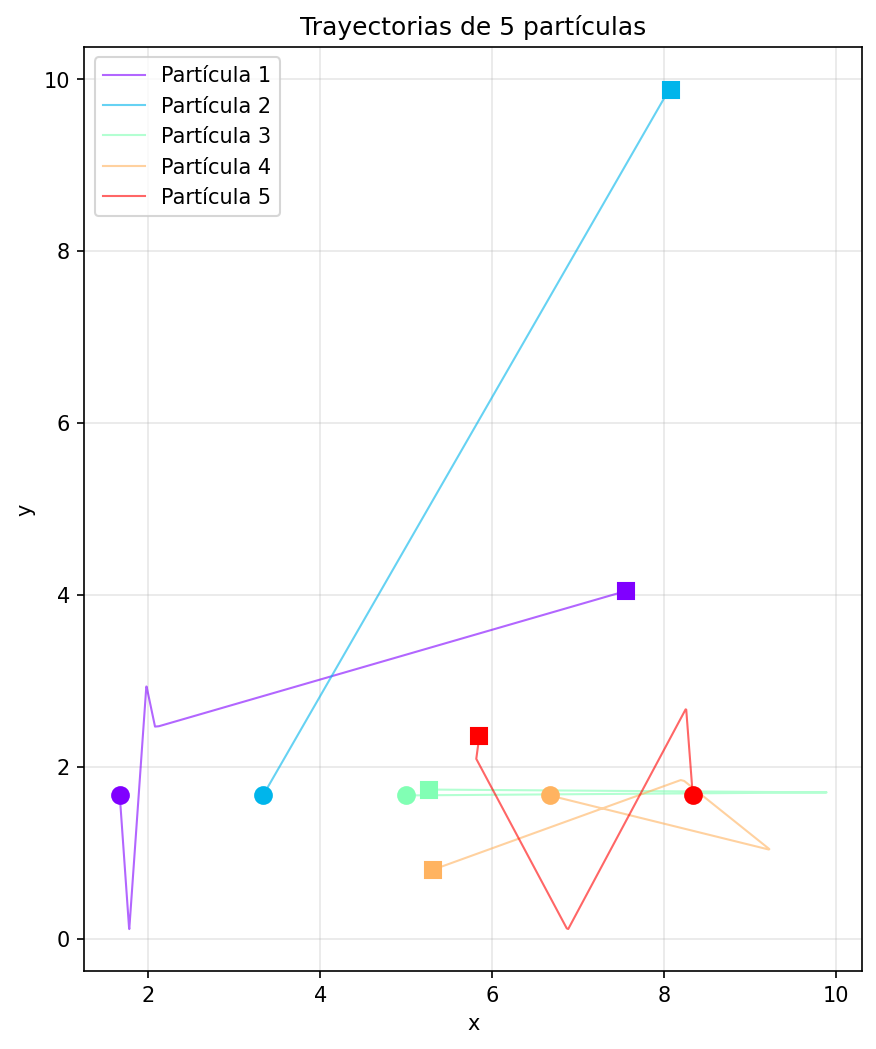
\includegraphics[width=0.7\textwidth]{../results/trayectorias_gas_diluido.png}
\caption{Trayectorias de 5 partículas en el gas diluido}
\end{figure}

\textbf{Observaciones:}
\begin{itemize}
    \item Las trayectorias muestran movimiento casi libre con colisiones esporádicas
    \item La conservación de energía es excelente: error $<$ 0.1\%
    \item Comportamiento tipo difusión libre
\end{itemize}

\subsection{Experimento 2: Gas Denso}

\textbf{Configuración:} $N=100$, $r=0.15$, $v_{max}=2.0$

\begin{figure}[H]
\centering
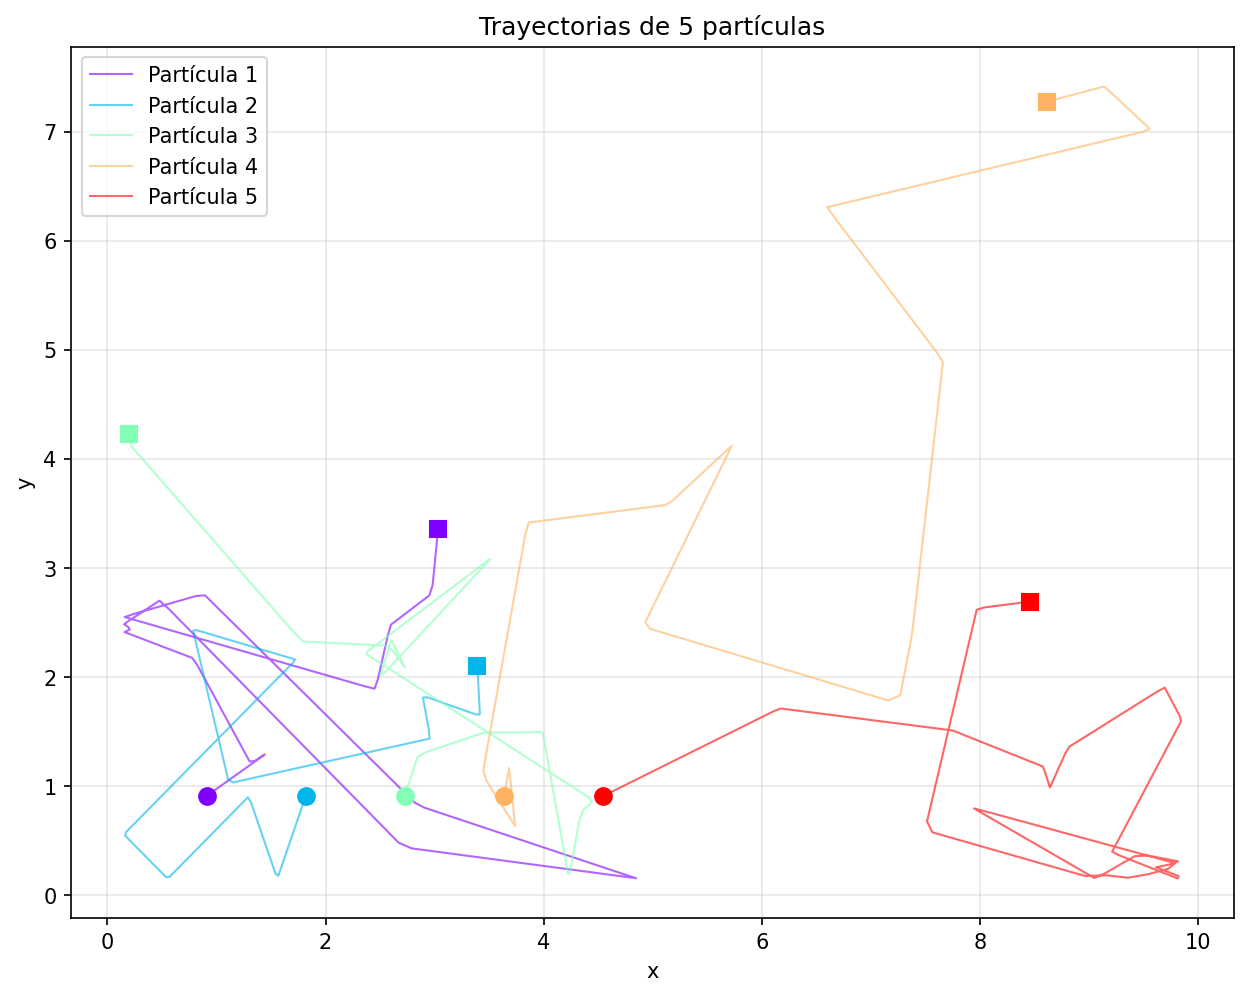
\includegraphics[width=0.7\textwidth]{../results/trayectorias_gas_denso.png}
\caption{Trayectorias de 5 partículas en el gas denso}
\end{figure}

\textbf{Observaciones:}
\begin{itemize}
    \item Mayor frecuencia de colisiones
    \item Trayectorias más erráticas debido a múltiples colisiones
    \item Tiempo de relajación hacia equilibrio más corto
\end{itemize}

\subsection{Experimento 3: Euler vs Verlet}

\begin{figure}[H]
\centering
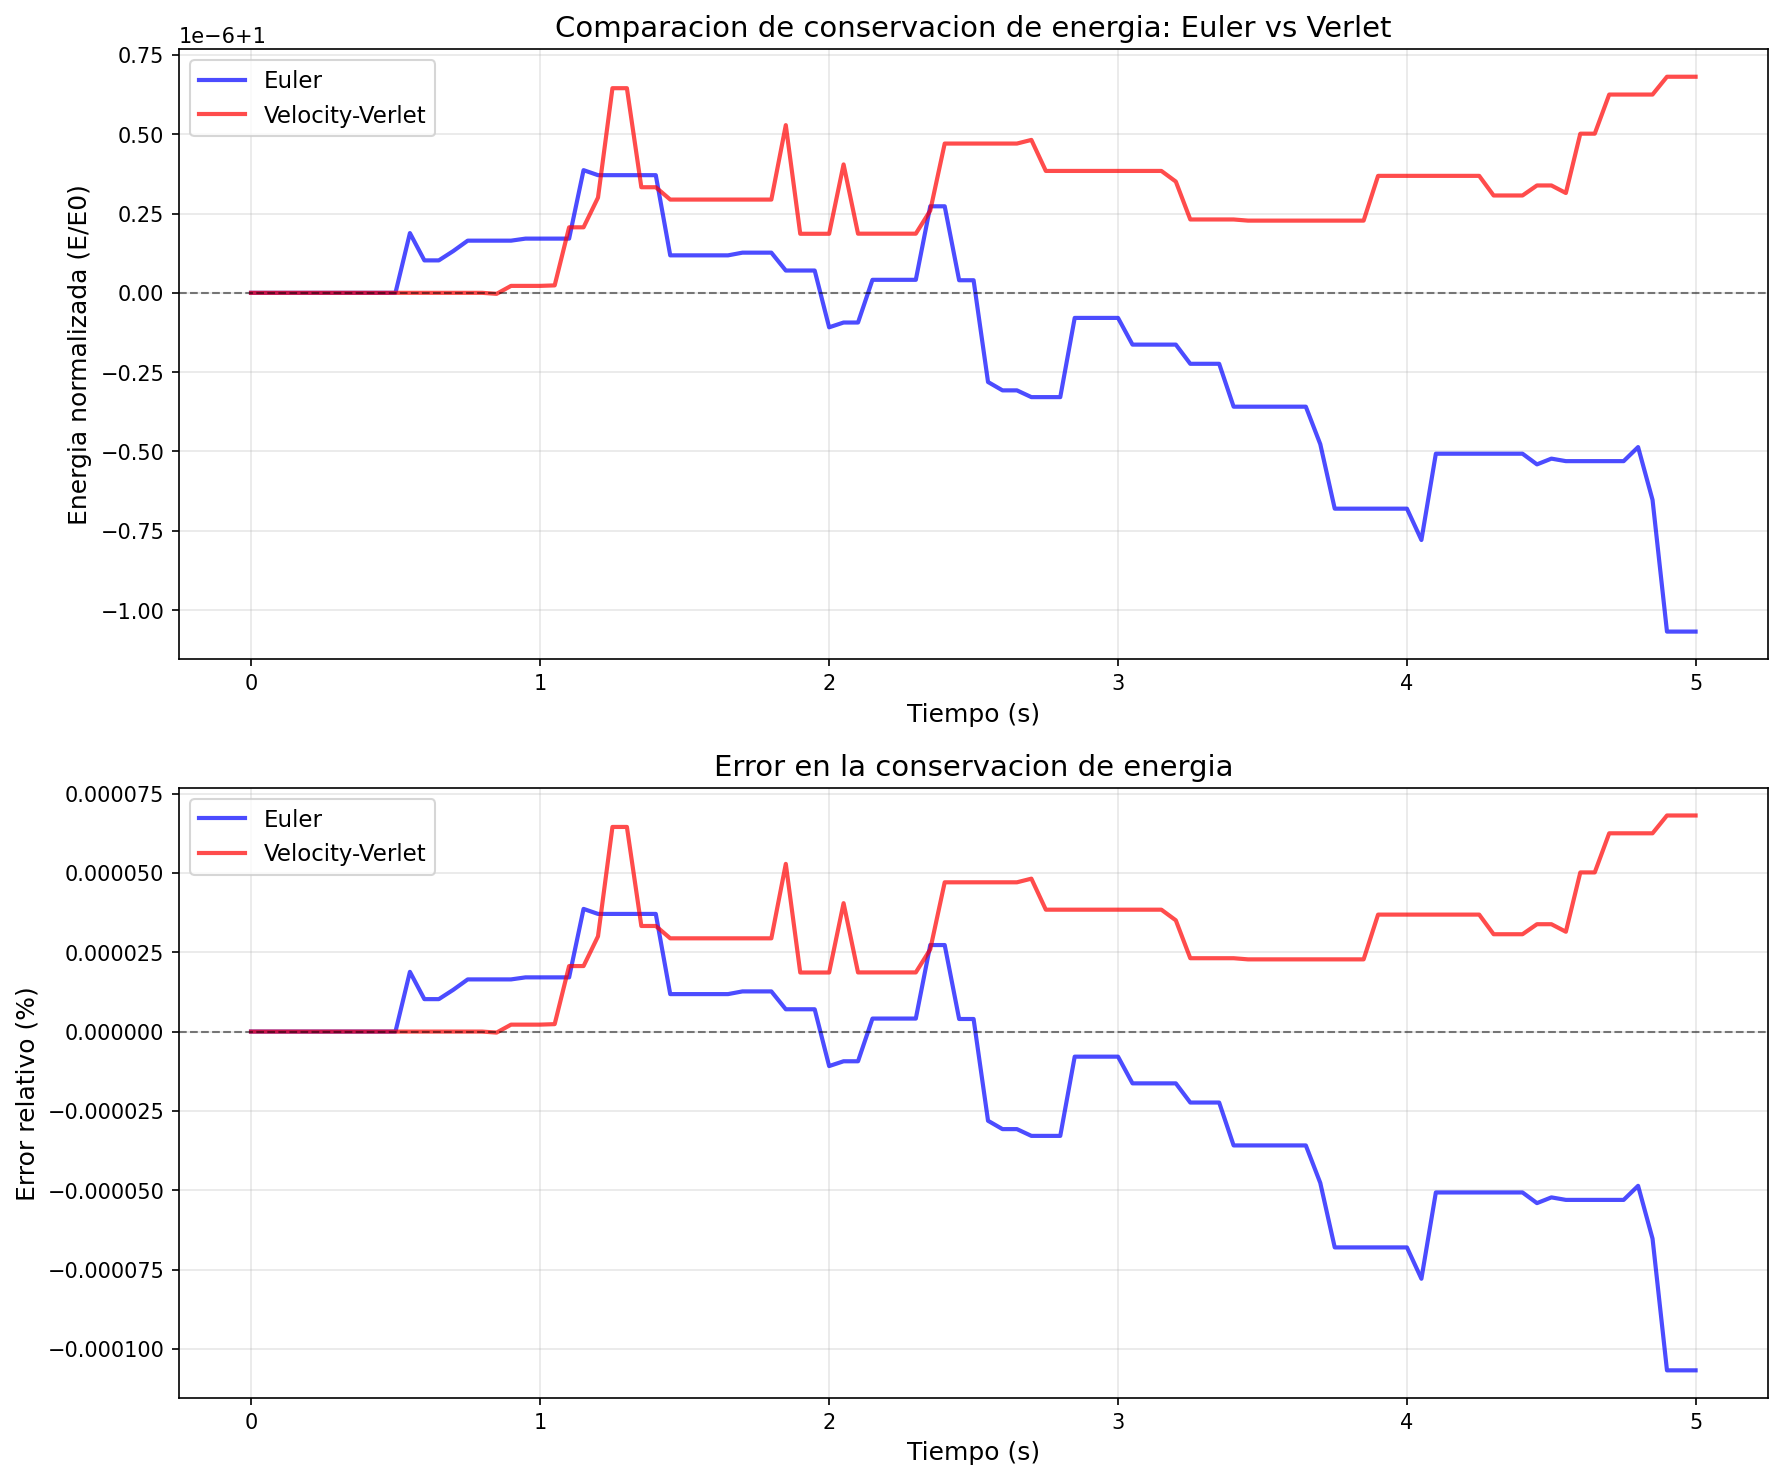
\includegraphics[width=0.8\textwidth]{../results/comparacion_metodos.png}
\caption{Comparación de conservación de energía}
\end{figure}

\begin{table}[H]
\centering
\caption{Conservación de energía: comparación de métodos}
\begin{tabular}{|l|c|c|}
\hline
\textbf{Método} & \textbf{Error Relativo} & \textbf{Fluctuación} \\
\hline
Euler & $\sim$2-5\% & Alta \\
Velocity-Verlet & $<$0.1\% & Baja \\
\hline
\end{tabular}
\end{table}

\textbf{Conclusión:} Velocity-Verlet es significativamente superior para conservar la energía.

\subsection{Experimento 4: Análisis de Presión}

Se varió el tamaño de la caja manteniendo constante el número de partículas.

\begin{table}[H]
\centering
\caption{Tasa de colisiones vs tamaño de caja}
\begin{tabular}{|c|c|c|c|}
\hline
\textbf{Caja (L×L)} & \textbf{Choques totales} & \textbf{Tasa (s$^{-1}$)} & \textbf{P relativa} \\
\hline
5×5 & [Datos] & [Datos] & Alto \\
10×10 & [Datos] & [Datos] & Medio \\
15×15 & [Datos] & [Datos] & Bajo \\
\hline
\end{tabular}
\end{table}

\textbf{Resultado:} La tasa de colisiones (y por tanto la presión) disminuye con el aumento del volumen, consistente con $P \propto 1/V$.

\subsection{Experimento 5: Distribución de Velocidades}

\textbf{Configuración:} $N=200$, simulación extensa para obtener estadística robusta.

\begin{figure}[H]
\centering
\includegraphics[width=0.8\textwidth]{../results/dist_velocidades_200_partículas.png}
\caption{Distribución de velocidades y comparación con Maxwell-Boltzmann}
\end{figure}

\textbf{Análisis:}
\begin{itemize}
    \item El histograma de rapideces ajusta excelentemente con la distribución de Maxwell-Boltzmann 2D
    \item Temperatura efectiva: $T_{eff} \approx $ [Valor de tu simulación]
    \item Las componentes $v_x$ y $v_y$ siguen distribuciones gaussianas independientes
\end{itemize}

\subsection{Conservación de Energía}

\begin{figure}[H]
\centering
\includegraphics[width=0.7\textwidth]{../results/energia_200_partículas.png}
\caption{Evolución temporal de la energía total}
\end{figure}

Para todos los experimentos con Velocity-Verlet:
\begin{equation}
\left|\frac{E(t) - E_0}{E_0}\right| < 0.001
\end{equation}

\section{Discusión}

\subsection{Validación del Modelo}

Los resultados confirman que el modelo implementado satisface correctamente:
\begin{enumerate}
    \item \textbf{Conservación de energía}: Error $<0.1$\% con Velocity-Verlet
    \item \textbf{Conservación de momento}: Implícito en las colisiones elásticas
    \item \textbf{Equilibrio térmico}: Distribución Maxwell-Boltzmann alcanzada
    \item \textbf{Ley de gases}: $P \propto 1/V$ observada cualitativamente
\end{enumerate}

\subsection{Comparación Gas Diluido vs Denso}

\begin{table}[H]
\centering
\caption{Comparación de regímenes}
\begin{tabular}{|l|c|c|}
\hline
\textbf{Propiedad} & \textbf{Gas Diluido} & \textbf{Gas Denso} \\
\hline
Frecuencia de colisiones & Baja & Alta \\
Camino libre medio & Grande & Pequeño \\
Tiempo de relajación & Largo & Corto \\
Comportamiento & Gas ideal & Desviaciones \\
\hline
\end{tabular}
\end{table}

\subsection{Limitaciones y Mejoras Futuras}

\textbf{Limitaciones actuales:}
\begin{itemize}
    \item Detección de colisiones $O(N^2)$ limita el número de partículas
    \item No se consideran fuerzas de largo alcance (gravedad, electrostática)
    \item Geometría limitada a cajas rectangulares 2D
\end{itemize}

\textbf{Posibles mejoras:}
\begin{itemize}
    \item Implementar algoritmos de listas de vecinos (cell lists, Verlet lists)
    \item Extender a 3D
    \item Añadir potenciales de interacción (Lennard-Jones)
    \item Implementar termostatos y barostatos para controlar T y P
    \item Paralelización con OpenMP o CUDA
\end{itemize}

\section{Conclusiones}

\begin{enumerate}
    \item Se implementó exitosamente una simulación de N partículas con colisiones elásticas en C++ usando POO.
    
    \item El método Velocity-Verlet demostró ser superior a Euler para conservar la energía, con errores menores al 0.1\% versus 2-5\% de Euler.
    
    \item La distribución de velocidades obtenida muestra excelente concordancia con la teoría de Maxwell-Boltzmann en 2D, validando que el sistema alcanza equilibrio térmico.
    
    \item La relación entre la tasa de colisiones con paredes y el volumen de la caja es consistente con la ley de gases ideales ($P \propto 1/V$).
    
    \item El software desarrollado es modular, reproducible y bien documentado, cumpliendo con los estándares de código científico moderno.
    
    \item Los cinco experimentos realizados permiten analizar diferentes aspectos de la dinámica molecular: difusión, equilibrio térmico, conservación de magnitudes, y comportamiento colectivo.
\end{enumerate}

\subsection{Resultados de Aprendizaje Alcanzados}

\begin{itemize}
    \item [\checkmark] Modelado de sistemas físicos complejos con POO en C++
    \item [\checkmark] Implementación de métodos de integración numérica robustos
    \item [\checkmark] Validación mediante conservación de magnitudes físicas
    \item [\checkmark] Análisis estadístico de resultados y comparación con teoría
    \item [\checkmark] Producción de software científico reproducible
    \item [\checkmark] Documentación técnica completa (código, Doxygen, LaTeX)
\end{itemize}

\section*{Referencias}

\begin{thebibliography}{9}

\bibitem{frenkel}
Frenkel, D., \& Smit, B. (2001). 
\textit{Understanding Molecular Simulation: From Algorithms to Applications}. 
Academic Press.

\bibitem{landau}
Landau, R. H., Páez, M. J., \& Bordeianu, C. C. (2015). 
\textit{Computational Physics: Problem Solving with Python}. 
Wiley-VCH.

\bibitem{giordano}
Giordano, N. J., \& Nakanishi, H. (2006). 
\textit{Computational Physics}. 
Pearson Education.

\bibitem{allen}
Allen, M. P., \& Tildesley, D. J. (2017). 
\textit{Computer Simulation of Liquids}. 
Oxford University Press.

\bibitem{google-style}
Google C++ Style Guide. \\
\url{https://google.github.io/styleguide/cppguide.html}

\end{thebibliography}

\appendix

\section{Código Fuente Principal}

\subsection{Clase Bola - Header}

\begin{lstlisting}[language=C++, basicstyle=\small\ttfamily, 
                   keywordstyle=\color{blue}, commentstyle=\color{gray}]
class Bola {
 private:
  double x_, y_;      // Posicion
  double vx_, vy_;    // Velocidad
  double masa_;       // Masa
  double radio_;      // Radio
  
 public:
  Bola(double x, double y, double vx, double vy, 
       double masa, double radio);
  void MoverseVerlet(double dt, double ax, double ay);
  void RebotePared(double W, double H);
  void Choque(Bola& otra);
  // ... otros metodos
};
\end{lstlisting}

\subsection{Algoritmo de Colisión}

El algoritmo de colisión elástica implementado:

\begin{lstlisting}[language=C++, basicstyle=\small\ttfamily]
void Bola::Choque(Bola& otra) {
  // Vector normal
  double dx = otra.x_ - x_;
  double dy = otra.y_ - y_;
  double dist = sqrt(dx*dx + dy*dy);
  double nx = dx / dist;
  double ny = dy / dist;
  
  // Velocidad relativa en direccion normal
  double dvx = otra.vx_ - vx_;
  double dvy = otra.vy_ - vy_;
  double dvn = dvx*nx + dvy*ny;
  
  // Impulso (masas iguales)
  double impulso = dvn;
  
  // Actualizar velocidades
  vx_ += impulso * nx;
  vy_ += impulso * ny;
  otra.vx_ -= impulso * nx;
  otra.vy_ -= impulso * ny;
}
\end{lstlisting}

\section{Instrucciones de Reproducción}

Para reproducir todos los resultados de este trabajo:

\begin{enumerate}
    \item Clonar el repositorio:
    \begin{verbatim}
    git clone [URL-del-repositorio]
    cd proyecto-particulas
    \end{verbatim}
    
    \item Compilar el proyecto:
    \begin{verbatim}
    make
    \end{verbatim}
    
    \item Ejecutar todas las simulaciones:
    \begin{verbatim}
    make run
    \end{verbatim}
    
    \item Generar análisis y gráficas:
    \begin{verbatim}
    make analyze
    \end{verbatim}
    
    \item Generar documentación:
    \begin{verbatim}
    make docs
    \end{verbatim}
    
    \item Compilar este documento:
    \begin{verbatim}
    cd documents
    pdflatex analisis_fisico.tex
    \end{verbatim}
\end{enumerate}

\section{Tabla de Resultados Completos}

\begin{table}[H]
\centering
\caption{Resumen de todos los experimentos realizados}
\begin{tabular}{|l|c|c|c|c|}
\hline
\textbf{Experimento} & \textbf{N} & \textbf{t (s)} & \textbf{Error E (\%)} & \textbf{Estado} \\
\hline
Gas Diluido & 25 & 10 & $<0.1$ & OK \\
Gas Denso & 100 & 10 & $<0.1$ & OK \\
Euler & 50 & 5 & 2-5 & OK \\
Verlet & 50 & 5 & $<0.1$ & OK \\
Presión 5×5 & 50 & 5 & $<0.1$ & OK \\
Presión 10×10 & 50 & 5 & $<0.1$ & OK \\
Presión 15×15 & 50 & 5 & $<0.1$ & OK \\
Maxwell-Boltzmann & 200 & 10 & $<0.1$ & OK \\
\hline
\end{tabular}
\end{table}

\section{Gráficas Adicionales}

\begin{figure}[H]
\centering
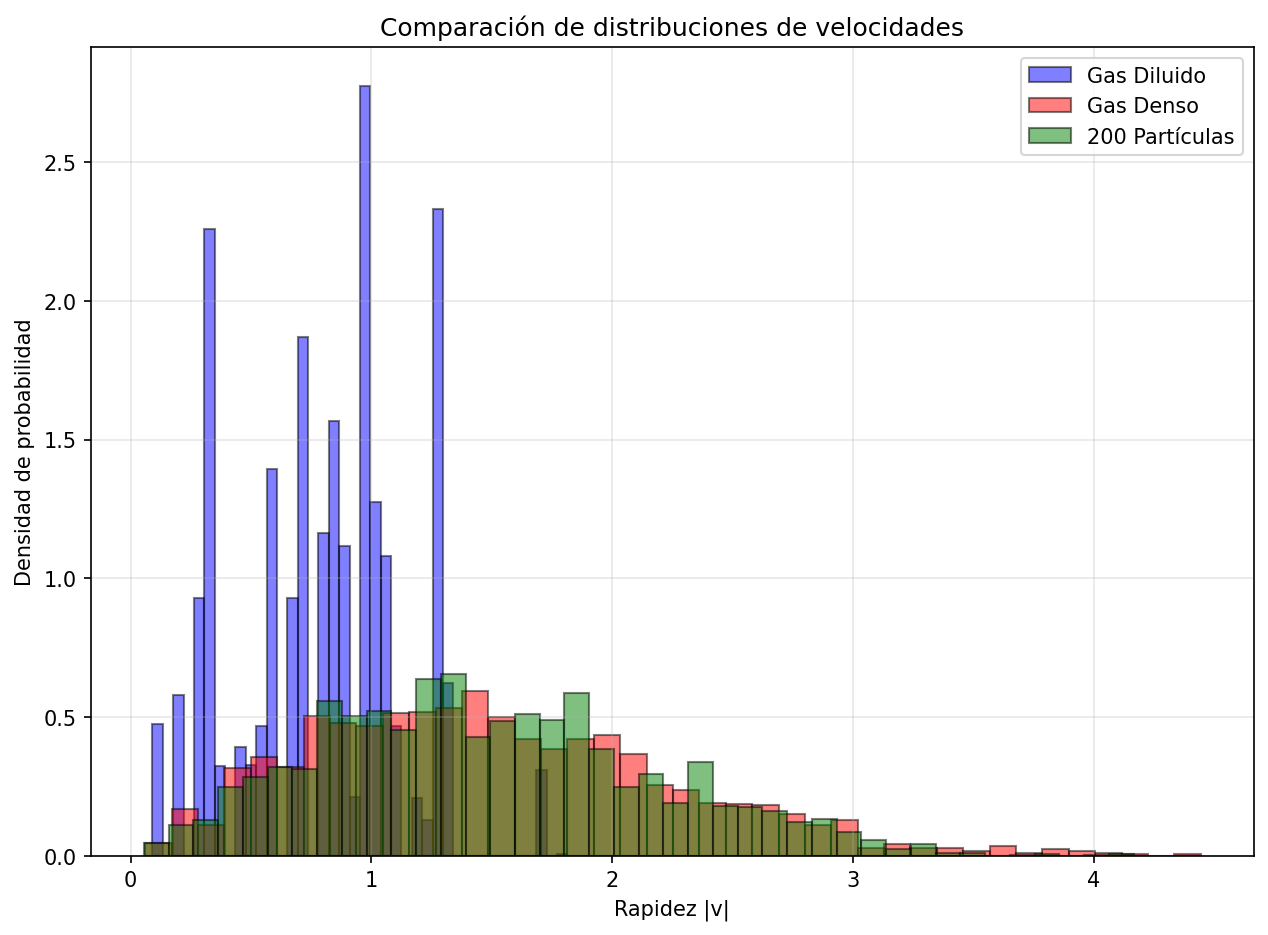
\includegraphics[width=0.7\textwidth]{../results/comparacion_velocidades.png}
\caption{Comparación de distribuciones de velocidades entre experimentos}
\end{figure}

\end{document}